\documentclass[a4paper,12pt]{article}

\usepackage[utf8]{inputenc}
\usepackage[ngerman]{babel}
\usepackage[T1]{fontenc}
\usepackage{graphicx}
\usepackage[cache=false]{minted}
\usepackage{dirtree}
\usepackage{biblatex}
\usepackage[strings]{underscore}
\addbibresource{literatur.bib}



\begin{document}
\begin{titlepage}
    \begin{center}
        \vspace*{1cm}
        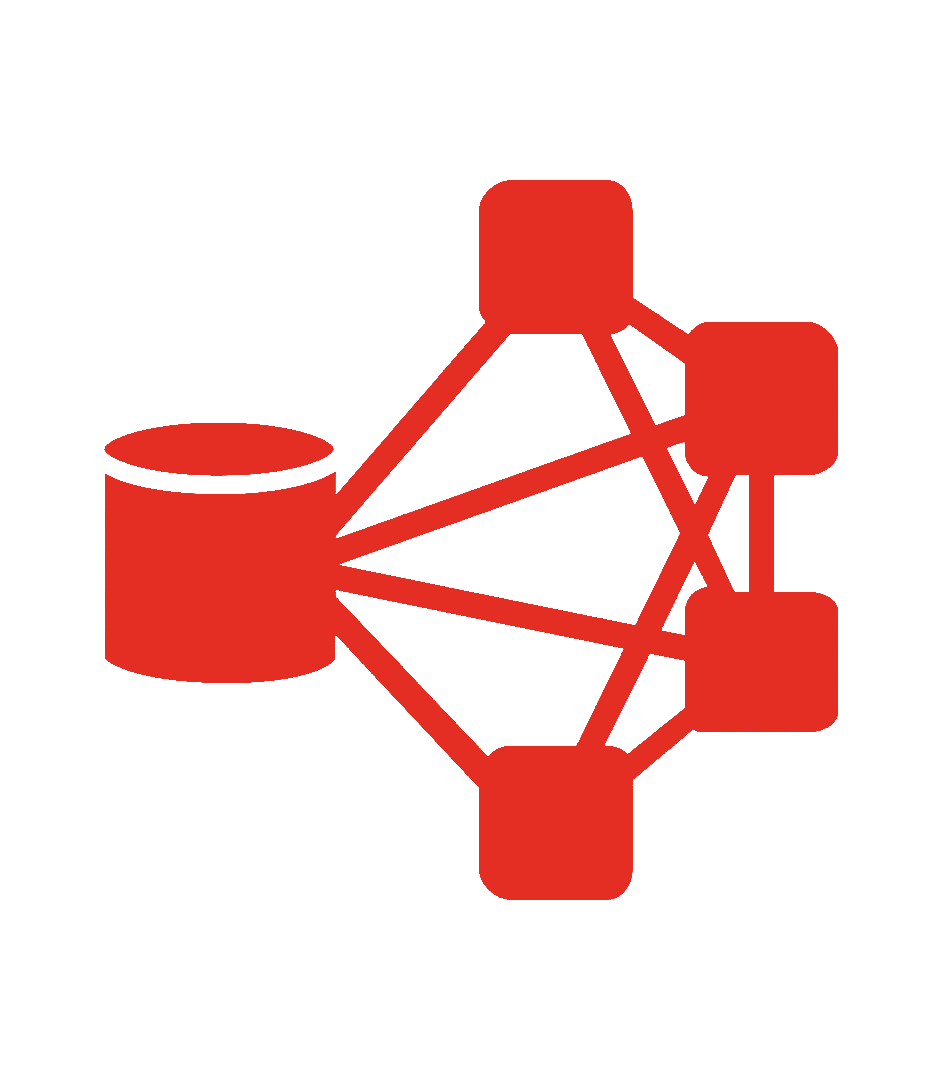
\includegraphics[width=10cm]{Logo.png}
        
        \textbf{\huge MapReduce-System}
        
        \vspace{0.5cm}
        NVS Projekt 2
                 
        \vspace{1.0cm}
    
        \textbf{Alexander Grill 5CHIF}
        
        \today
        
        \vfill
                 
                 
        \vspace{0.5cm}
                 
        Informatik\\
        HTBLUvA Wr.Neustadt\\
        Österreich\\

                 
    \end{center}
\end{titlepage}  
\newpage
\tableofcontents
\newpage


\section{Einführung}
In diesem Kapitel werden die Gründe der Umsetzung und das Thema, worum es in dieser Arbeit geht, genau erläuter. Es wird auch
darauf eingegangen, welche Thematiken das Projekt umfassen soll und wie sich die Benotung auseinander setzt.

\subsection{Vorwort}
Der Virus "COVID-19" war im Jahr 2020 für die gesamte Bevölkerung auf der Erde eine rießengroße Herausforderung. Die Situation änderte sich am Begin im daruffolgendem Jahr 2021 nicht, 
deshalb beschloss die Bundesregierung weiter Maßnahmen, Ausgangsbeschränkunge, Grenzkontrollen, FFP2-Maskenpflicht und weitere Regeln die, die Bevölkerung einzuhalten hat. Alle Schüler in Österreich müssen die Schule 
blockweiße besuchen. Nur mit einem davor verpflichtetenden Schnelltest und FFP2-Maske dürfen sie die Schule betrehten. Da die Projektarbeiten im ersten Semster dementsprechend gut ausgefallen sind, beschloss Herr Professor 
Kolousek, dass Schüler in den fünften Klassen im Fach NVS statt der Praktischen Arbeit und dem Theorie Test eine Projektarbeit über den Semsterstoff machen müssen. Folgendessen muss die Dokumentation, über das gewählte Thema, dementsprechend einen
weiteren Umfang umfassen als beim ersten Projekt im ersten Semster. Im praktischen Teil geht es in diesem Projekt, darum ein Map-Reduce System in Kombination mit Server-Client Kommunikation zu implementier. Im theoretischen Teil, werden die Grundlagen die für die 
Umsetzung relevant sind erklärt. Zusätzlich beinhaltet dies auch sämtliche Abschnitte wie, die Source Code Dokumentation, Abläufe, Erklärung bezgl. MapReduce-System, Aufbau und Anwendungsfälle.
\begin{description}
    \item[Die zu erreichende Note hängt prinzipiell von der] ~\par
    \begin{itemize}
        \item Beispielkategorie
        \item Art der Kommunikation
        \item Funktion, Umfang und Tiefe der Implementierung
        \item Fehlerbehandlung
        \item Ausgaben, Einhaltung der Coding Conventions, Kommentare
        \item Repository: Commits, Issues
        \item Ausarbeitung
        \item Einhaltung der Richtlinien
      
    \end{itemize} 
\end{description}
\subsection{Motivation}
In diesem NVS Projekt geht es darum, ein MapReduce-System mit der Programmiersprache C++ unter Linux mittels g++ Compilier umzusetzten.
Im kurzem zusammengefasst soll eine große Menge an komplexen, unstrukturierten und eine Art von aufwendigen Daten verarbeitet werden. 
Das heißt es sollen Daten, die planlos abgespeichert sind, zusammengefasst werden, sodass diese wieder ihren Nutzen oder Sinn erbringen. Diese können
dann für weiter Verarbeitungsschritte oder Datenanalysen verwendet werden. Die Daten werden am Beginn in kleiner Packete aufgeteilt und diese werden identifiziert mit einem eindeutigen
Schlüssel. In der nächste Phase werden die einzelnen Packete parallel von unterschiedlichen, getrennten und unabhängigen Prozesse zusammengefasst. Danach werden die gruppierten Daten wieder 
einen Schlüssel zugeordnet, sodass diese wieder zusammengefasst und minimiert werden. Die Kommunikation zwischen den einzelnen Knoten, soll in dieser Arbeit mittel Server-Client Kommunikation passiern.
Der Server hört auch einem Port ab, ob sich ein Client damit verbinen möchte, wenn eine Verbindung aufgebaut werden kann, soll die Splittung der Daten passier, daraufhin soll das Resultat weiter an dem Server gegeben werden, bis 
alle Daten vereint auf dem Master Server liegen. Die bearbeitetn Daten werden schlussendlich in einem JSON-File abgespeichert.
\section{Aufgabenstelllung}
Diese Kapitel umfasst die genaue Erläuterung der Aufgabenstelllung, als auch die Themenbereiche die dieser Projektarbeit. Darüber hinaus wird auch über die Idee der Umsetzung geschrieben.

\subsection{Erläuterung der Aufgabenstellung}
Ziel ist es das eine Menge von unstrukturierten Daten, so verarbeitet werden, dass diese danach wieder in ordnungsgemäßer Struktur vorliegen. Zuerste müssen die Daten aufgeteilt werden. Sie werden in einer Key-Value Form abgepeichert, somit kann
der Value, also der abgespeicherte Datensatz, mittels Key eindeutig identifiziert werden. Nachdem die Daten zusammengefasst vorliegen, werden sie in nächste Schritt auf einzelne Knoten aufgeteilt. Diese erlangen von den einzelenen Clients die Daten in Key-Value Form und fassen diese wieder zusammen, bis die Daten zu einem Master Knoten ankommen und dort schlussendlich in geordneter Form darliegen.
Die Aktionen, der Datenverarbeitung verläuft ständig unter paralleler Abfolge, die Aufgaben werden aufgeteilt und gleichlaufen auf verscheidenen Knoten aufgeteilt.

\subsection{Idee}
Das Projekt ist so aufgebaut, das es acht oder mehr Clients gibt, zwei Slave Server und einen Master Server. Ein Benutzer(Client) kann einen beliebige Anzahl von Zeichenketten, die er dem Programm beim Aufruf mitübergibt, erzeugen und diese werden dann in einer Datei abgespeichert. Zuästzlich wird dem Benutzer auch angeboten dem Speichertort der Datei selbst auszuwählen. Nachdem die ungeordneten Daten in einer Datei 
abspeichert sind, beginnt die nächste Phase des Map-Reduce System. Die Datei wird zeilenweise durchgegangen. Die Zeichenketten werden in einem Art Dictionary als Key-Value Form abspeichert, daduch kann jeder eingefügte Datensatz identifiziert werden. Wenn der Datensatz in diesem Dictionary schon existiert, dann wird der Value, der als Counter festlegt wie oft die Zeichenfolge im Text vorkommt, um eins erhöht. Nachdem kompletten Durchlauf der Datei sind alle Daten
in diesem Dictionary abspeichert. Dadurch, dass mehrere Clients das System zum gleichen Zeitpunkt unabhängig voneinander nutzen können, wird das durchforsten der Datei von anderen Prozessen nicht beeinflusst. Nachdem ein Prozess mit der Datenabspeicherung fertig ist, sendet er die Daten an den jeweiligen Slave Server der zu diesem Zeitpunkt nicht beschäftigt ist. Wenn der Server von einer gewissen Anzahl von Clients die Daten bekommt, beginnt er danach mit der Map Phase. An dieser Stelle werden
die gesendetet Daten wieder per Key zusammengefasst und strukturiert. Die Abarbeitung erfolgt auch in diesem Fall parallel zu einem weiter Slave Knoten, der die selbe Art und Weise der Datenverarbeitung nutzt. Schlussendlich wird das Result an den Master Server geschickt. Letzendlich bringt dieser all seine empfangen Daten in eine Struktur, die im Nachhinein für Datenanalysen eingesetzt werden können.
\subsection{Themenbereiche}
\begin{description}
    \item[Diese Arbeit umfasst folgende Thematiken] ~\par
    \begin{itemize}
        \item Grundlagen und Basiskonzepte, Nachrichtenübertragung, Netzarchitektur
        \item Internetprotokoll
        \item Transportprotokolle
        \item Prozesse und Threads
        \item Synchronisation und parallele Programmierung
        \item Kommunikation, Serverprogrammierung, verteilte Systeme
        \item TCP/IP Programmierung      
    \end{itemize} 
\end{description}
\newpage
\section{Grundlagen}

\subsection{Was ist ein MapReduce System?}
Das Verfahren wurde 2004 von Google entwickelt für die Indexierung von Webseiten. Das Framework wird bei Datenbanken eingesetzt und dient zur Verarbeitung von großen, komplexen, unstrukturierte Datenmengen.
Dieses Verfahren findet Anwendung für BigData und Datawarehouse, weil in solchen Fällen große Datenmengen in kürzester Zeit mittels Software verarbeitet, analysiert, aggregiert als auch kompremiert werden. 
Map Reduce parallelisiert die Bearbeitung, durch die Verteilung auf mehrere gleichzeitig auszuführende Tasks. Der Grund, warum dieses Framework solche Datenmengen verarbeiten kann ist, weil die Aufgaben auf mehreren Rechnern aufgeteilt werden. Jeder einzelne Rechner startet Prozesse, die Parallel die Daten verarbeitet und auswertet.
Ein einzelner Rechner stoßt schnell an seine Grenzen, deshalb ist die Verarbeitung von Daten, mittels mehreren Knoten sehr effizient und bietet eine bessere Performance.
Das Verfahren wurde in vielen verschiedenen Verfahren eingesetzt wie zum Beispiel für die Indizierung von Webseiten, nach einer Suchanfrage mit beliebigen Zeichenketten, ebenso im Umfeld von Google News wird MapReduce verwendet. Andere große Internetfirmen wie Yahoo, die ebenfalls das Verfahren für die Indexierung von Webseiten verwenden, 
als auch Facebook verwendet das System, um Spam Messages zu minimierung und die Ads zu optimieren. Wohingegen Amazon das Verfahren für das Clustering der Produket verwendet

\subsection{Map und Reduce}
Die beiden Grundfunktionen des Verfahrens sind Map und Reduce. Sie sorgen für die Aufteilung der Aufgaben in kleinere parallelisierten Arbeitspakete und führen am Ende die Ergebnisse zusammen. Bei großen relationalen Datenbanken und komplexen Queries lassen sich typische Problem, bezglüch Verarbeitung von großen Datenmengen beseitigen.
Die Map Funktion, verteilt die Aufgaben an unterschiedlichen Knoten eines Clusters. Die Reduce Funktion sortier die verfassten Ergebnisse und fügt sie am Ende wieder zusammen.
Die Funktionen Map und Reduce werden vom User bereitgestellt, weil diese schließlich zu den bereitgestellten Daten passen müssen.
\cite{mrsystem}
\newpage

\subsection{Ablauf}

\begin{figure}[h]
    \centering
    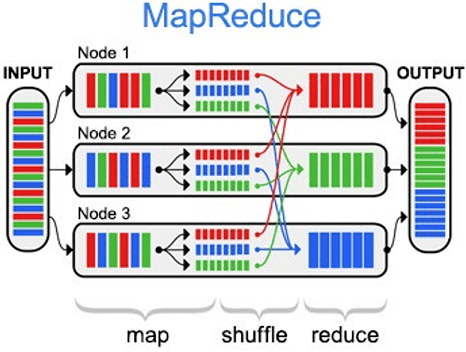
\includegraphics[width=6.1cm]{mapreduce.png}
\end{figure}
\begin{description}
    \item[Das Verfahren verläuft durch folgende Schritte:] ~\par
    \begin{itemize}
        \item Split
        \begin{itemize}
            \item{Die bereitgestellten Daten werden aufgeteilt. Jeder Datensatz darin ist identifiziert durch
            einen Schlüssel-Wert. Diese Datenmenge wird nun in kleinere Datenmengen aufgeteilt
            und vom Master an die verfügbaren Knoten verteilt.}
        \end{itemize}
        \item Map 
        \begin{itemize}
            \item{Nun wendet jeder Knoten auf die Daten die Map-Funktion an, die schließlich Key/Value Paare zurückgibt. Diese Ergebnisse werden zwischengespeichert.}
        \end{itemize}
        \item Shuffel
        \begin{itemize}
            \item{Bei diesem Schritt geht es darum den reduce-Knoten, die entsprechenden Daten zuzuteilen.
            Diese Zuteilung entspricht einer Fragmentierung.
            Hierbei wird den Knoten, die reduce ausführen, ein Key zugeteilt. Diese Knoten holen sich
            dann die bereits durch Map entstandenen Datensätze mit diesem Key und wenden reduce an.}
        \end{itemize}
        \item Reduce
        \begin{itemize}
            \item{Grundsätzlich ist die Aufgabe dieser Funktion, die Key/Value Paare anhand des Schlüssels
            zusammenzufassen und dabei die Summe der einzelnen Values zu bilden. Demnach ist die
            Ausgabe der Reduce-Funktion wieder ein Key/Value Paar mit dem gleichen Aufbau wie vor
            der Verarbeitung.
            Dies ermöglicht es, dass reduce mehrere Male angewendet werden kann, bis schließlich alle
            Daten gesammelt wurden.}
        \end{itemize}
    \end{itemize} 
\end{description}

\subsection{Vorteile Nachteile eines Map-Reduce Systems}
Map Reduce bietet eine Menge an Vorteilen, gegenüber den klassischen Verfahren der Datenverarbeitung, wie
sie in den relationalen Datenbanksystemen verwendet werden. \\ \\
Ein wesentlicher Vorteil ist, dass für die
Verwendung eines solchen System ein einfacher normaler Rechner benötigt wird und keine Highend-Server. Ein Cluster-Verbund für die parallelisiert
Datenverarbeitung kann bei Notwendigkeit ohne großen Aufwand realisiert werden. Ein Cluster-Verbund ist ein Netzwerk, das aus mehreren Rechner besteht die gleichzeit miteinander verbunden sind 
und sich Daten austauschen. Aus diesem Grund ist ein MapReduces-System sehr kostensparsam und kann mit wenig Know-How und Erfahrungen umgesetzt und
schlussendlich in Verwendung gebracht werden. \\ \\
Ein weiterer Vorteil ist auch die Skalierbarkeit. Da die Daten auf den jeweiligen Knoten
aufgeteilt werden, bietet das System eine zuverlässige Ausfallstoleranz und Verfügbarkeit, denn wenn ein Knoten ausfallen sollte, werden die Daten einfach an einem
anderen Knoten und dort verarbeitet, somit läuft das System zu jederzeit in einem stabilen Zustand. \\ \\
Durch die parallelisierte Verarbeitung von Daten ist dieses Verfahren deutlich effizienter und perfomanter als die Datenverarbeitung
in relationalen Datenbanken. Im Terabyte-Bereich dauert das Verfahren oft nur Minuten, im Petabyte-Bereich Stunden, wobei andere Systeme deutlich mehr Zeit und Ressourcen für die Verarbeitung
benötigen.\\ \\
Während die Berechnungen schnell gehen, dauert der Datenzugriff länger als bei anderen Methoden. 
Die Daten müssen erst über das Netzwerk gestreamt werden. Dabei ist die Netzanbindung der Flaschenhals, vor allem im Hinblick auf die sehr unterschiedlichen Rechner innerhalb des Clusters und deren unterschiedliche schnelle Netzanbindung.\\ \\
Um die Geschwindigkeit zu erhöhen, kann ein Cluster ausschließlich aus High-End-Servern bestehen. In diesem Fall sind die Kosten für das MapReduce-Verfahren immens hoch.
\cite{vorteil/nachteilemrsystem}
\subsection{Parallel Programming}

\subsection{Kommunikation}
Das Prinzip der Kommunikation im Internet ist, dass man strikt sein sollen beim Senden der Daten und tolerant beim Empfängen. Der Zweck einer Kommunikation sind die Interoperabilität, das bedeutet
das mehrere Systeme die aus Rechner bestehen in der Lage sind Daten untereinander auszutauschen, und die Fehlertolaranz, das bedeutet das die Daten durch festegelegte Regeln übertragen werden aber beim Empfangen in einer
gewünschen Form umgewandelt werden können.

\begin{description}
    \item[Beziehungen zwischen den einzelnen Knoten] ~\par
    \begin{itemize}
        \item one-to-one
        \begin{itemize}
            \item{Ein Knote kommuniziert mit einen anderen Knoten}
        \end{itemize}
        \item one-to-many
        \begin{itemize}
            \item{Ein Knoten spricht mit mehreren Knoten und alle lauschen und hören zu. Diese Art von Kommunikation zwischen den Rechner nennt man multicast}
        \end{itemize}
        \item one-to-any
        \begin{itemize}
            \item{Ein Knoten spricht mit mehreren Knoten, jedoch betrifft das nur einen Knoten von mehreren.}
        \end{itemize}
        \item many-to-one
        \begin{itemize}
            \item{Mehrere Knoten sprechen zu einen konkreten Knoten}
        \end{itemize}
        \item many-to-many
        \begin{itemize}
            \item{Mehrer Knoten kommuniziert mit mehreren anderen Knoten.\\}
        \end{itemize}
    \end{itemize} 
\end{description}
Weiters ist beim Datenautausch wichtig festzuhalten, in welche Richtung die Daten übertragen werden. Mittel simplex werden die Daten nur in eine Richtung übertragen. 
Bei half-duplex werden die Daten ebenso in eine Richtung übertragen, jedoch kann die Richtung in der Übertragen wird änderen. Bei der Variante duplex werden die Daten in beide Richtungen übertragen wie im TCP Protokoll realisiert, werden zwei Streams
zur Verfügung gestellt um Daten zu senden und zu empfangen.\\\\\\\\
Im Grunde genommen unterscheidet man zwischen verbindungsorientierter und verbindungsloser Kommunikation. Bei der verbindungsorientierter Kommunikation wird eine Verbindung zwischen zwei Knoten aufgebaut, danach werden Daten ausgetauscht und zum Schluss kommt es zur
Verbindungsabbau. Wohingegen bei der verbindungsloser Kommunikation nur die Datenübertragen werden und keine Verbindung aufgebaut und abgebaut wird. Es ist in der Regel effizienter, aber es wird nicht sichergestellt ob die Daten wirklich beim Empfänger angekommen sind.\\ \\
Bei der Kommunikation werden auch Nachrichten ausgetauscht, die zum Aufbau, der Überwachung und dem Abbau einer Verbindug notwendig sind. Man spricht von in-bank signalling, es wird ein gleicher logischer Kanal wie Nutzdaten und Steuerungsdaten verwendet, oder out-of-band signalling, hier wird ein getrennter logischer Kanal verwendet. Es gibt einen
physischen Kanal der in mehrere logische Kanäle unterteilt sind. \\ \\
Für die Kommunikation benötigt man auch festgelegte Regeln, die für eine Kommunikation notwendig sind, darunter versteht man den Begriff Protokoll. Das betrifft das Format der Nachrichten, Reihenfolge der Nachrichten und die Spezifikation der Fehlersituation. Es gibt zustandsbehaftete und zustandlose Protokolle. zustandsbehaftete Protokolle sind, jene bei denen die Nachrichten
vom Zustand der zuvor gesendete Nachrichten abhängt. Bei dem zustandlos Protokol heißt, die Nachrichten sind unabhängig von zuvor gesendeten Nachrichten.\\\\
Im Informationaustausch spielt auch der Begriff Session eine wichtige Rolle. Dieser beschreibt eine feste Beziehung zwischen kommunizierenden Prozessen mit vereinbarten Eigenschaften wie Namen, Ressourcen, Charakteristika. Dadurch bildet sich ein gemeinsamer Zustand zwischen dein einzelnen Prozessen. Um sicherzustellen welcher Knoten welcher ist und welche Rechte dieser hat 
bei der Kommunikation mit anderen hat, werden Mechanismen zu Authentifikation und Autorisierung. Bei HTTP sieht die Kommunikation folgendermaßen aus, ein Client der mittels Browser eine Seite aufruft sendet einen Request an den Server, dieser überprüft die Daten der Anfragen und welche Daten der Client benötigt und sendet den Client danach mittels Respone die angefragten Daten zurück.\\
Wird die Seite neu geladen so verschwinden auch die Daten die in einem Cache zwischengespeichert sind und für weitere Aktionen relevant sind. Dies kann oft zu Problem führen, deshalb wird ein sogenanter Session-Cookie verwendet, in dem Daten abgelegt werden, die in einer Session entstehen und für weitere Tätigkeiten relevant sind und in diesem abgespeichert werden.\\ \\
Protokolle sind hierachisch angeordnet, dass hat den Vorteil, dass mit Problemen zwischen den unterschiedlichen Protokollen besser umgehen kann und jede Schicht nur wissen muss was mit der darunterliegenden Schicht zu tun ist und wie Daten an die darüberliegenden Schicht geben kann. Die Schichten können auch ausgetauscht werden.
\\\\
Die Kommunikation kann durch unterschiedlichen Stillen durchgeführt werden wie zum Beipsiel wird ein gemeinsamer genutzer Knoten verwendet und auf diesem zugegriffen auf dem alle Daten abgespeichert werden, wie es bei Datenbanken der fall ist, beim Versenden von Nachrichten spricht man von nachrichten-orientierte Kommunikation, beim Aufruf einer Funktion oder Methoden die auf einem Client abgespeichert sind
spricht man von Entfernte Funktionsaufrufe bzw. Entfernte Methodenaufrufe, wenn Daten verarbeite werden wenn sie eintreffen spricht man von stream-orientierter Kommunikation.\\\\
Ein Nachrichtenautausch kann entweder synchron oder asynchron passierten. Bei einer synchronen Austausch wird die Operation begonnen, wenn der Sender die Nachricht initiert hat und der Empfänger bereit ist die Nachricht zu empfangen. Wobei bei einer asynchronen Nachrichtenaustauch, der Sender die Nachrichten unabhängig, ob der bereit ist oder nicht. 
\begin{description}
    \item[Semantik der Nachrichtenübermittlung] ~\par
    \begin{itemize}
        \item no-wait-send
        \begin{itemize}
            \item{Der Sendeprozess wartet lediglich bis die Nachricht im Transportsystem zum Absenden bereitgestellt ist.}
        \end{itemize}
        \item synchronization send
        \begin{itemize}
            \item{Der Sendeprozess wartet bis die Nachricht vom Empfangsprozess entgegengenommen worden ist.}
        \end{itemize}
        \item remote-invocation send
        \begin{itemize}
            \item{Der Sendeprozess wartet bis die Nachricht vom Empfangsprozess verarbeitet und beantwortet worden ist.\\\\\\\\\\}
        \end{itemize}
    \end{itemize} 
\end{description}
Die Datenübertragen in einem Netzwerk kann transient sein(Message Passing), das heißt beide Kommunikationspartner müssen online sein, weil das Kommunikationssystem speichert Nachrichten nur solange, wie die
sendende und die empfangene Operation ausgeführt wird, oder Persistent(Message Queueing), darunter versteht man das Kommunikationssystem speichert Nachrichten bis diese vollständig an den Empfänger ausgeliefert wurden.\\\\
Musterlösungen einer Datenübertragung kann sein request/response(A sendet an B, B sendet an A), oneway(A sendet an B, A sendet an B), batching(Zusammenfassung von oneway Nachrichten) und publish/subscribe. Daten können durch zweit verscheiden Möglichkeiten interoperable übertragen werden, nämlich Daten werden ganz einfach in ein maschinenunabhängiges Format transformiert oder Empfänger muss sich um eine notwendige Konvertierung kümmern. Im ersten Fall müssen beide Kommunikationspartner
die Daten so umwandelen, sodass diese für sie verständlich sind und im zweiten Fall spezifiziert der Sender den Datentyp aus einer Liste von vorgegebenen Datentypen.
\cite{communication1}
\subsection{TCP/IP}




\section{Umsetzung}

\subsection{Aufbau}

\subsection{Source Code Dokumentation}

\subsection{Kommandozeilenparameter}

\subsection{Konsolenausgabe}


\subsection{Verwendete Bibliotheken}

\section{Anwendungsfälle}

\section{Schlusswort}

\section{Literatur}

\printbibliography
\end{document}
